\section{Software Performance} \label{chapter3:software-performance}

\comment{TODO Introduction}

Programming started with a sequential nature.
The Moore's law \cite{Moore1965} and Dennard's MOSFET scaling \cite{Dennard2007} were wrongly interpreted to promise the exponential evolution in the sequential performance of the processing unit.
 % Programming started with a very sequential nature, as Moore's law \cite{Moore1965} was wrongly interpreted as an exponential evolution in the sequential performance of the processing unit.

% TODO Dennard scaling broke down \cite{Dennard2007}

\sout{The first models of computation, like the Turing machine and lambda-calculus, were sequential and based on a global memory state.
A formalism was missing to represent concurrent computations.
This section presents the most important works on formalisms for parallel computation.
They tackled the problems of determinacy, state synchronization and correctness of execution in a formalism based on a network of concurrent processes, asynchronously communicating via messages.
This section first presents the works on the programming models based on this formalism.
Then it presents the huge improvements we recently witnessed in the field of distributed stream processing due to the need of performance from the web to process large stream of requests,}

\subsection{Parallel Programming}

\comment{Introduction}

\begin{center}
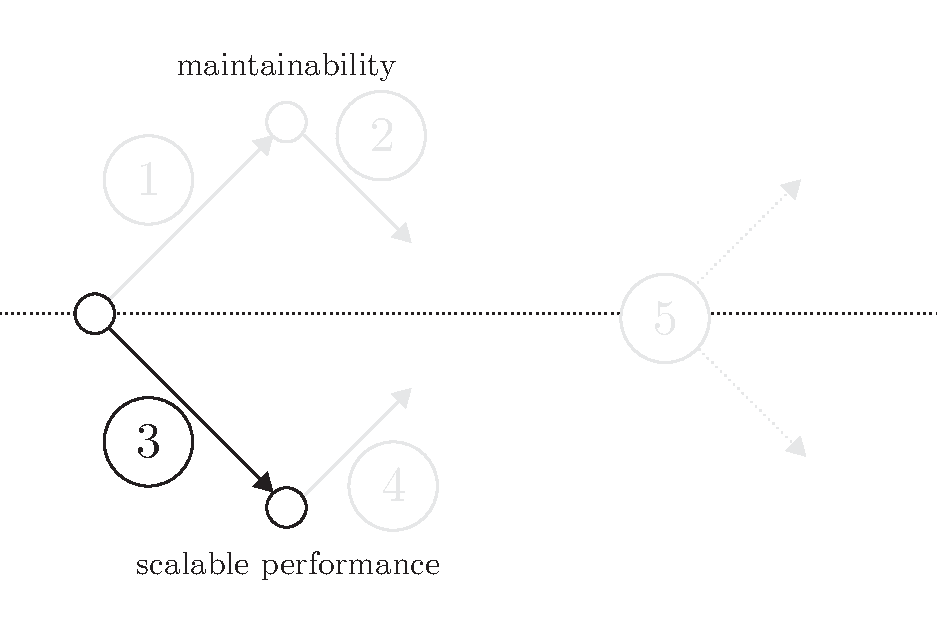
\includegraphics[width=0.6\textwidth]{../ressources/state-of-the-art-3.pdf}
\end{center}

Include in this section :\\
Flynn's taxonomy \cite{Flynn1972}\\
+ Actor models\\
+ Scala / Akka\\
+ Play - on top of akka (Asynchronous)\\
\\

Scala is an attempt at unifying the object model and functional programming \cite{Odersky2004}.
% It proposes an actor approach in its design.
Akka\ftnt{http://akka.io/} is a framework based on Scala, to build higly scalable and resilient applications.


\subsubsection{Execution Causality}

\nt{Causal ordering of execution, instead of global ordering
Causality / Concurrent programming / Asynchronism / Message-passing / Synchronization ...}

Causal ordering of execution, instead of global ordering, lead to concurrent programming, and with some memory synchronization to parallel programming.

% All these early work adopted concurrent composition by default, instead of sequential composition, to adapt to the very concurrent nature of real parallel machines.
% However, sequential programming is still the default.
% Concurrent composition is yet still to be widely accepted, as stated by Reed \cite{Reed2012}.
% \comment{TODO rewrite this paragraph}
\sout{
% The Actor Model uses asynchronous communications, while $\pi$-calculus uses synchronous communications.
% Synchronous communications are deterministic.
% The message sent needs to be received to continue the execution on both ends.
Because of the synchronous communication used by $\pi$-calculus, the concurrent executions and the communications are both deterministic.
Therefore, the result of the concurrent system is assured to be deterministic.
The correctness of the execution of deterministic systems is guaranteed.
% Determinism is a wanted property to assure the correctness of the execution.
}

\sout{
On the other hand, the asynchronous communications used by Actors are non-deterministic.
The message sent can take an infinite time to be received.
Therefore, the result of the concurrent system is not assured to be deterministic.}

But the communication in reality are subject to various faults and attacks \cite{Lamport1982}.
And the wait required by synchronous communications negatively impact performances of the system because of the difference of latency between communication, and execution.
The Actor model was explicitly designed to take these physical limitations in account \cite{Hewitt1977a}.
The non-determinism in the asynchronous communications is hidden by the organization of the system.
The total ordering of execution possible with synchronous communication is too strong a requirement for correctness.
\nt{emphasize next sentence}
As Lamport showed \cite{Lamport1978}, and Reed related later \cite{Reed2012}, causal order is sufficient to build a correct distributed system.
% The non-determinism in the asynchronous communications is hidden by the organization of the system.
The ordering of execution is only local to an \comment{entity}, while between \comment{entities}, execution is causally ordered.
The execution will either terminate correctly, or not terminate at all because of a failure in the communications.

\sout{Eventually, following works adopted asynchronous communications as it is hardly realistic to build a distributed system based on synchronous communications.}




% Asynchronous communications are less expressive than synchronous ones \cite{PALAMIDESSI2003}.

% Pi-calculus is a synchronous paradigm which contains an asynchronous fragment.\cite{PALAMIDESSI2003}
% (Boudol, G. (1992). Asynchrony and the π-calculus (note). Rapport de Recherche  1702, INRIA, Sophia-Antipolis,
% Honda, K. and Tokoro, M. (1991).  An object calculus for asynchronous communication. In America, P., editor, Proceedings of the European Conference on Object-Oriented Programming (ECOOP), volume 512 of Lecture Notes in Computer Science, pages 133–147. Springer-Verlag)


% The asynchronous pi-calculus defined by Honda and Tokoro in 1991 led to Pict, a programming language\cite{Pierce2000}.




% There was firstly theories, and models for concurrent computation.
% The main problem was determinism.
% In a sequential machine, the non-determinism of the physical world is hidden by the sequentiality of the machine.
% However, in concurrent computation, the order of communication cannot be assured the way the order of statements is assured in a sequential machine.
% We observe local non-determinism.
% However, to conserve an apparent determinism, causal ordering is sufficient.




\subsubsection{State Independence}


\sout{As demonstrated by the theory, concurrency boils down to causality expressed with message passing.
There exist several programming model over this theoretical view.}

\paragraph{Independent Processes}

The theory advocates asynchronous message-passing, but it doesn't precise the granularity of the communicating entities.
In the Actor Model, everything is an actor, even the simplest types, like numbers, similarly in OOP, everything is an object.
In practice, this level of granularity is unachievable due to overhead from the asynchronous communications.
Most implementations adopt a granularity on the process or function level.

% concurrent programming
The first concept using message passing was the coroutine.
% It influenced many following works.
Conway defines coroutines as an autonomous program which communicate with adjacent modules as if they were input and output subroutines \cite{Conway1963}.
It is the first definition of a pipeline to implement multi-pass algorithms.
Similar works include the Communicating Sequential Processes (CSP) \cite{Hoare1978, Brookes1984}, and the Kahn Networks \cite{Kahn1974, Kahn1976}.

% Hoare presented the Communicating Sequential Processes (CSP) \cite{Hoare1978, Brookes1984}.
% These processes are executed concurrently, and communicates events via named channels.
% The evolutions of this model were influenced by, and influenced the work of Milner that led to $\pi$-calculus.

% Similarly, Kahn developed the Kahn Networks \cite{Kahn1974, Kahn1976}, following the work of Conway on coroutines.
% They are explicitly parallel coroutines separated by bounded FIFO streams for communication.

These programming models don't allow to dynamically modify the topology of the application.
Coroutines and processes are defined statically in the source of the application.
We shall come back to this limitation later in this thesis in chapter \ref{chapter5}.

Erlang is a functional concurrent language designed by Ericsson to operate telecommunication devices \cite{JoeArmstrong,Nelson2004} % Nelson2004 is not very good, find another better citation.

% The shared-nothing architecture \cite{Stonebraker1986}.

As we saw in last section, higher-level programming is helping modularity.
The absence of this feature in the concurrent programming model is a limitation.
On of the instrumental gaol of this thesis is to allow to bring higher-level programming in parallel programming, without the need for manual synchronization, as we will see in the next section.

\subparagraph{PGAS}

Sharing resources eventually limits scalability, hence distribution of the memory is unavoidable.
The Partitioned Global Address Space (PGAS) model replaces the need for a common memory store.
It provides the developers with a uniform memory access on a distributed architecture.
Each computing node executes the same program, and provide its local memory to be shared with all the other nodes.
The PGAS programming model assure the remote accesses and synchronization of memory across nodes, and enforces locality of reference, to reduce the communication overhead.
% This model is a SPMD : Single Program Multiple Data.
Known implementation of the PGAS model are 
Chapel\cite{Chamberlain2007},
X10 \cite{Charles2005}.
Unified Parallel C \cite{El-Ghazawi2006},
CoArray Fortran \cite{Numrich1998} and
OpenSHMEM \cite{Chapman2010}.

These programming models are promising.
However, they focus rather on scientific application with intensive computing such as matrix multiplication, and leave out streaming applications, such as web services.

\paragraph{\sout{Programming languages}} \label{chpater3:concurrent-programming:programming-languages}

% Scala / Akka / Erlang

\sout{Some programming languages features message-passing and isolation of actors directly to give the responsibility to developers to assure high parallelism.
To some extent, these languages succeeded in industrial contexts.
However, they largely remain elitist solutions for specific problems more than a general, and accessible tool.
I present some examples below.}


The field of concurrent programming is so vast it is impossible to relate here every of its branch.
The previous examples are only the best known.
The next focus focuses on streaming real-time applications.




\comment{transition on lazy evaluation equivalence to stream. lazy evaluation + side effects + concurrency = streams}

\paragraph{Stream Processing Systems} \label{chapter3:parallel-execution:stream-processing}

All the solutions previously presented are designed to build general distributed systems.
We focus on real-time applications as defined by \cite{Hansen1978}.
A real-time application must respond to a variety of simultaneous requests within a certain time.
Otherwise, input data may be lost or output data may lose their significance.
Such applications are often connected to the internet and use the web as an interface, which implies to process high volumes streams of requests.
Moreover, because these systems are key to business, their reliability and latency are of critical importance.
These requirements are challenging to meet in the design of such system.
It present the state of the art to design such systems with these challenging requirements.


% \textit{
% From a language designer's point of view, real-time
% programs have these characteristics:
% \begin{enumerate}
% \item A real-time program interacts with an environ-
% ment in which many things happen simultaneously at
% high speeds.
% \item A real-time program must respond to a variety
% of nondeterministic requests from its environment. The
% program cannot predict the order in which these requests
% will be made but must respond to them within certain
% time limits. Otherwise, input data may be lost or output
% data may lose their significance.
% \item A real-time program controls a computer with a
% fixed configuration of processors and peripherals and
% performs (in most cases) a fLxed number of concurrent
% tasks in its environment.
% \item A real-time program never terminates but contin-
% ues to serve its environment as long as the computer
% works. (The occasional need to stop a real-time program,
% say at the end of an experiment, can be handled by ad
% hoc mechanisms, such as turning the machine off or
% loading another program into it.)
% \end{enumerate}
% }


\subparagraph{Dataflow pipeline} \label{chapter3:software-efficiency:dataflow-pipeline}

An alternative model to process data stream efficiently is the pipeline architecture.
It inspires from dataflow to integrate the two conflicting programming paradigms into one.

SEDA is a precursor in the design of pipeline-based architecture for real-time applications for the internet \cite{Welsh2001}.
It organizes an application as a network of event-driven stages connected by explicit queues.
It is based on previous works \cite{Gribble2001,Pai1999}.

Several projects followed and adapted the principles in this work.
StreaMIT is a language to help the programming of large streaming application \cite{Thies2002}.
Storm \cite{Toshniwal2014} is designed by and used at Twitter calculate metrics on streams of tweets such as the trending topics.
% It is only one example of industrial practical application, among many others.
Among other works, there are CBP \cite{Logothetis2010} and S4 \cite{Neumeyer2010}, that were designed at Yahoo, Millwheel \cite{Akidau2013} designed at Google and Naiad \cite{Murray2013} designed at Microsoft.

Similarly to the programming models presented in section \ref{chpater3:concurrent-programming:programming-languages} these frameworks are elitist and not accessible to a large community of developers.
Indeed, the pipeline architecture presents a distributed storage, which is hardly compatible with the best practices.
It impacts maintainability.
For this reason, there are some works on reconciling the concurrent programming models with the modular programming model favoring maintainability.

+ Spidle: A DSL approach to specifying streaming applications dataflow like


  (From the paper : Making state explicit for imperative big data processing)
  + MapReduce       map/reduce   |   Stateless dataflow
  + DryadLINQ       functional   |   Stateless dataflow
  + Spark           functional   |   Stateless dataflow
  + CIEL            imperative   |   Stateless dataflow
  + Hadoop          map/reduce   |   Stateless dataflow
  + Incoop          map/reduce   |   Incremental dataflow
  + Nectar          functional   |   Incremental dataflow
  + CBP             dataflow     |   Incremental dataflow
  + Comet           functional   |   Batched dataflow
  + D-Streams       functional   |   Batched dataflow
  + Naiad           Dataflow     |   Batched dataflow
  + Storm, S4       dataflow     |   Continuous dataflow
  + SEEP            dataflow     |   Continuous dataflow
  + Piccolo         imperative   |   Parallel in-memory
  + SDG             imperative   |   Stateful dataflow

% Dataflow
%   CBP          Incremental dataflow \cite{Logothetis2010}
%   S4           Continuous dataflow \cite{Neumeyer2010}
%   Storm        Continuous dataflow \cite{Toshniwal2014}
%   Millwheel    Continuous dataflow \cite{Akidau2013}
%   SEEP         Continuous dataflow \cite{Fernandez2013}
%   Naiad        Batched dataflow \cite{Murray2013}



\comment{Transition on the limitations of software parallelism}

\subsubsection{Elitism of Parallel Programming}

\comment{TODO}

\comment{TODO Transition on the maintainability improvements}

\subsection{Maintainability Improvements}

\comment{Introduction}

\begin{center}
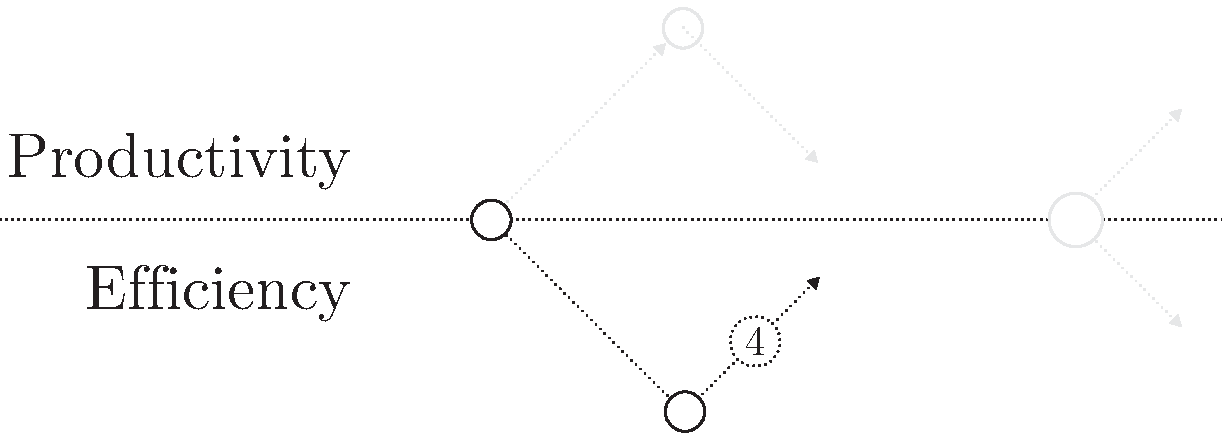
\includegraphics[width=0.6\textwidth]{../ressources/state-of-the-art-4.pdf}
\end{center}

\subsubsection{Design Patterns}

\nt{The following paragraph is not very clear}
As we explained in the previous sections, the two different organization, modular and parallel, seems intuitively incompatible.
However, it might be possible to find specific organizations that are both modular and parallel, and fit both requirements of maintainability and performance.
% fit both concerns for particular cases.

Algorithmic skeletons are general computational framework for distributed computing proposing predefined patterns that fit certain type of problems \cite{Cole1988, Dean2008, McCool2010, Gonzalez-Velez2010}.
A developer expresses its problem as a specific case of a skeleton.
It simplifies the design and implementation of the communications, hence the developer can focus on its problem independently of the distributed communications, and their performance overhead.

\nt{Link with DSMS}
As there is similtudes between SQL-like languages, functional structures, and algorithmic skeletons, the latter can be seen as a tentative to merge the more descriptional features of the former into imperative programming.
Indeed, among the Algorithmic skeletons, we can cite Map / reduce, which are functional structures, but are somehow equivalent to the select and aggregate functions of SQL.
The pipeline architecture for data stream processing presented in section \ref{chapter3:software-efficiency:dataflow-pipeline} can be considered as algorithmic skeletons.

However, they introduce limitations and difficulties, as the developer must fit its problem into the skeletons.
% One of this difficulties, it that a common memory is impossible to use.
Developers needs to think in terms of message passing instead of a global memory, which, as we saw in previous section, is incompatible with best practices.

\subsubsection{Granularity}

Another approach in an industrial context is the Service Oriented Architectures (SOA).
It allows developers to express an application as an assembly of services connected to each others.
It shows well the difference between Information Hiding Principles and Separation of Concerns, as a service doesn't encapsulate a design choice, but a specific task.
SOA is in contradiction with the former, but consistent with the latter.

More recently, in the web service development communities, emerged the term of microservices, following the trends of SOA.
It to choose and deacrease the granularity of the fitting between modular organization and parallel execution.
Using Microservices implies that software developers can manage the two organizations at a sufficiently fine level.
As said in section \ref{chpater3:concurrent-programming:programming-languages} and \ref{chapter3:software-efficiency:dataflow-pipeline}, it is an elitist point of view.
Most developers are unable to manage efficiently the two organizations.

\textbf{++}

\nt{TODO EJB}

\subsubsection{Lack of Higher-Order Programming}

Moreover, in these solutions, higher-order programming is impossible.
As we showed earlier in section \ref{chapter3:software-design:programming-models:functional-programming}, higher-order programming is important for modular design and maintainability.
The next section present some work on compiling from one organization into the other.
By keeping the modular programming model, the compilation approach allows higher-level programming. 

\paragraph{Transistion : these methods doesn't allow higher-order programming, which is required for good modularity. WHY ?}

\nt{TODO link with 3.1}

\endinput

\subsection{Concurrency Theory} \label{chapter3:parallel-execution:concurrency-theory}

The mathematical models are a ground for all following work on concurrent programming, we briefly explain them in the next paragraphs.
There are two main formal models for concurrent computations.
The Actor Model of C. Hewitt and the Pi-calculus of R. Milner.
Based on these definitions, we explain the importance of determinism for correctness, and the reasons that made asynchronous message-passing prevail.

% TODO illustration of cells, and draw an analogy between cells and actor model.
% Or something the actor models is based upon.

\subsubsection{Models}

\paragraph{Actor Model}

The Actor model allows to express the computation as a set of communicating actors \cite{Hewitt1973a, Hewitt1977, Clinger1981}.
In reaction to a received message, an actor can create other actors, send messages, and choose how to respond to the next message.
All actors are executed concurrently, and communicate asynchronously.
% The Actor model uses an asynchronous message-passing communication paradigm.
% The communication between two actors, the sender and the receiver, is a stream of discrete messages.
% The sender names the receiver actor when sending messages to be the recipient of these messages.
An asynchronous communication implies that the sender continues its execution immediately after sending the message, before receiving the result of the initiated communication.

The Actor model was presented as a highly parallel programming model, but intended for Artificial Intelligence purposes.
Its success spread way out of this scope, and it became a general reference and influence.
% For example, the Scala programming language features an actor approach to concurrency.

% More recent work of C. Hewitt on Actors is about ... \nt{TODO} \cite{Hewitt2007,Hewitt2007a}.

\paragraph{$\pi$-calculus}

R. Milner presented a process calculus to describe concurrent computation : the Calculus of Communicating Systems (CCS) \cite{Milner1975, Milner1980}.
It is an algebraic notation to express identified processes communicating through synchronous labeled channels.
% In CCS, process compose concurrently, communications are synchronous, and the topology is static.
The $\pi$-calculus improved upon this earlier work to allow processes to be communicated as values, hence to become mobile \cite{Engberg1986,Milner1992a,Milner1992}.
Therefore, similarly to Actors, in Pi-calculus processes can dynamically modify the topology.
However, contrary to the Actor model, communications in Pi-calculus are based on simultaneous execution of complementary actions, they are synchronous.


% Actors can create actors, pi-caclulys processes can replicate, and send processes through channel.
% Processes create a new processes on each instruction to continue the execution.!g systolic arrays

% Pi-calculus resembles to the actor model, but its algebraic nature led to a critical difference with the latter.
% Indeed, processes in the Pi-calculus communicate indirectly, through labeled ports, whereas actors communicate directly by naming the recipient actors.
% This difference allows multiple processes to listen in turns to the same channel, whereas the recipient of a message cannot change.

% I think this difference lead the Pi-calculus to be composable, whereas message-passing is not.
% Message-passing is not composable, whereas invocation is.
% The Actor model is not an ideal programming model, as non-composability makes difficult to reuse or extends existing components.
% A way to compose actors, is to send to an actor the name of the actor to respond to.
% It is similar in essence to the continuation concept.








\section{Reconciliations} \label{chapter3:reconciliations}
\nt{TODO title not clear enough}

\subsection{Contradiction}

The decomposition of an application into a pipeline, as shown in the two previous sections, is incompatible with the modular design advocated by the separation of concerns.
The problem of incompatibility between the modular design and the parallel execution of a pipeline architecture is the following.
There need to be a common understanding on the structure of the communication from one stage to the next.
The modular design defines that this common ground, the interface, be the most resilient possible to focus the evolution within a module.
While the pipeline architecture (and more generally the concurrent programming models) defines these interfaces as the communications between the stages of the execution.
With the evolution of the problem specification, when a stage needs to be modified, it is most likely that these changes will affect the previous or next stages.
% which will eventually change with the evolution of the problem specification.

Most project use languages supporting the modular design at the beginning, when they need to evolve the most.
They then switch to the pipeline architecture only when the requirement of performance overcomes the requirement of evolution.
Moreover, as the team knows that they will eventually throw away their code to upgrade it to a different paradigm, there is little effort to follow the best practice to make maintainable code.
It results in a large effort of development to compensate this rupture.
% This rupture between the two organization is not novel, and is at the center of a large body of work.
In this section, we present the state of the art to reconciliate the two organizations, and avoid this rupture.
First we see the design patterns to fit both organization onto a same source code.
Then we see the compilation tentatives to switch from one to the other.










TO READ :

Flynn's taxonomy
\cite{Flynn1972}

Streaming
\cite{Madsen2015}
\cite{Sun2015}

Map Reduce
\cite{Yao2015}


Web assembly
https://medium.com/javascript-scene/what-is-webassembly-the-dawn-of-a-new-era-61256ec5a8f6